\documentclass{article}
\usepackage{tikz}
\usetikzlibrary{shapes.geometric, arrows, positioning}

\tikzstyle{startstop} = [ellipse, minimum width=3cm, minimum height=1cm, text centered, draw=black, fill=red!30]
\tikzstyle{process} = [rectangle, minimum width=3cm, minimum height=1cm, text centered, draw=black, fill=blue!30]
\tikzstyle{decision} = [diamond, minimum width=3cm, minimum height=1cm, text centered, draw=black, fill=green!30]
\tikzstyle{note} = [rectangle, text width=5cm, text centered, draw=black, fill=yellow!30, rounded corners]
\tikzstyle{arrow} = [thick,->,>=stealth]

\begin{document}

\section*{Flowchart: Neural Network Training Process and Optimizations}

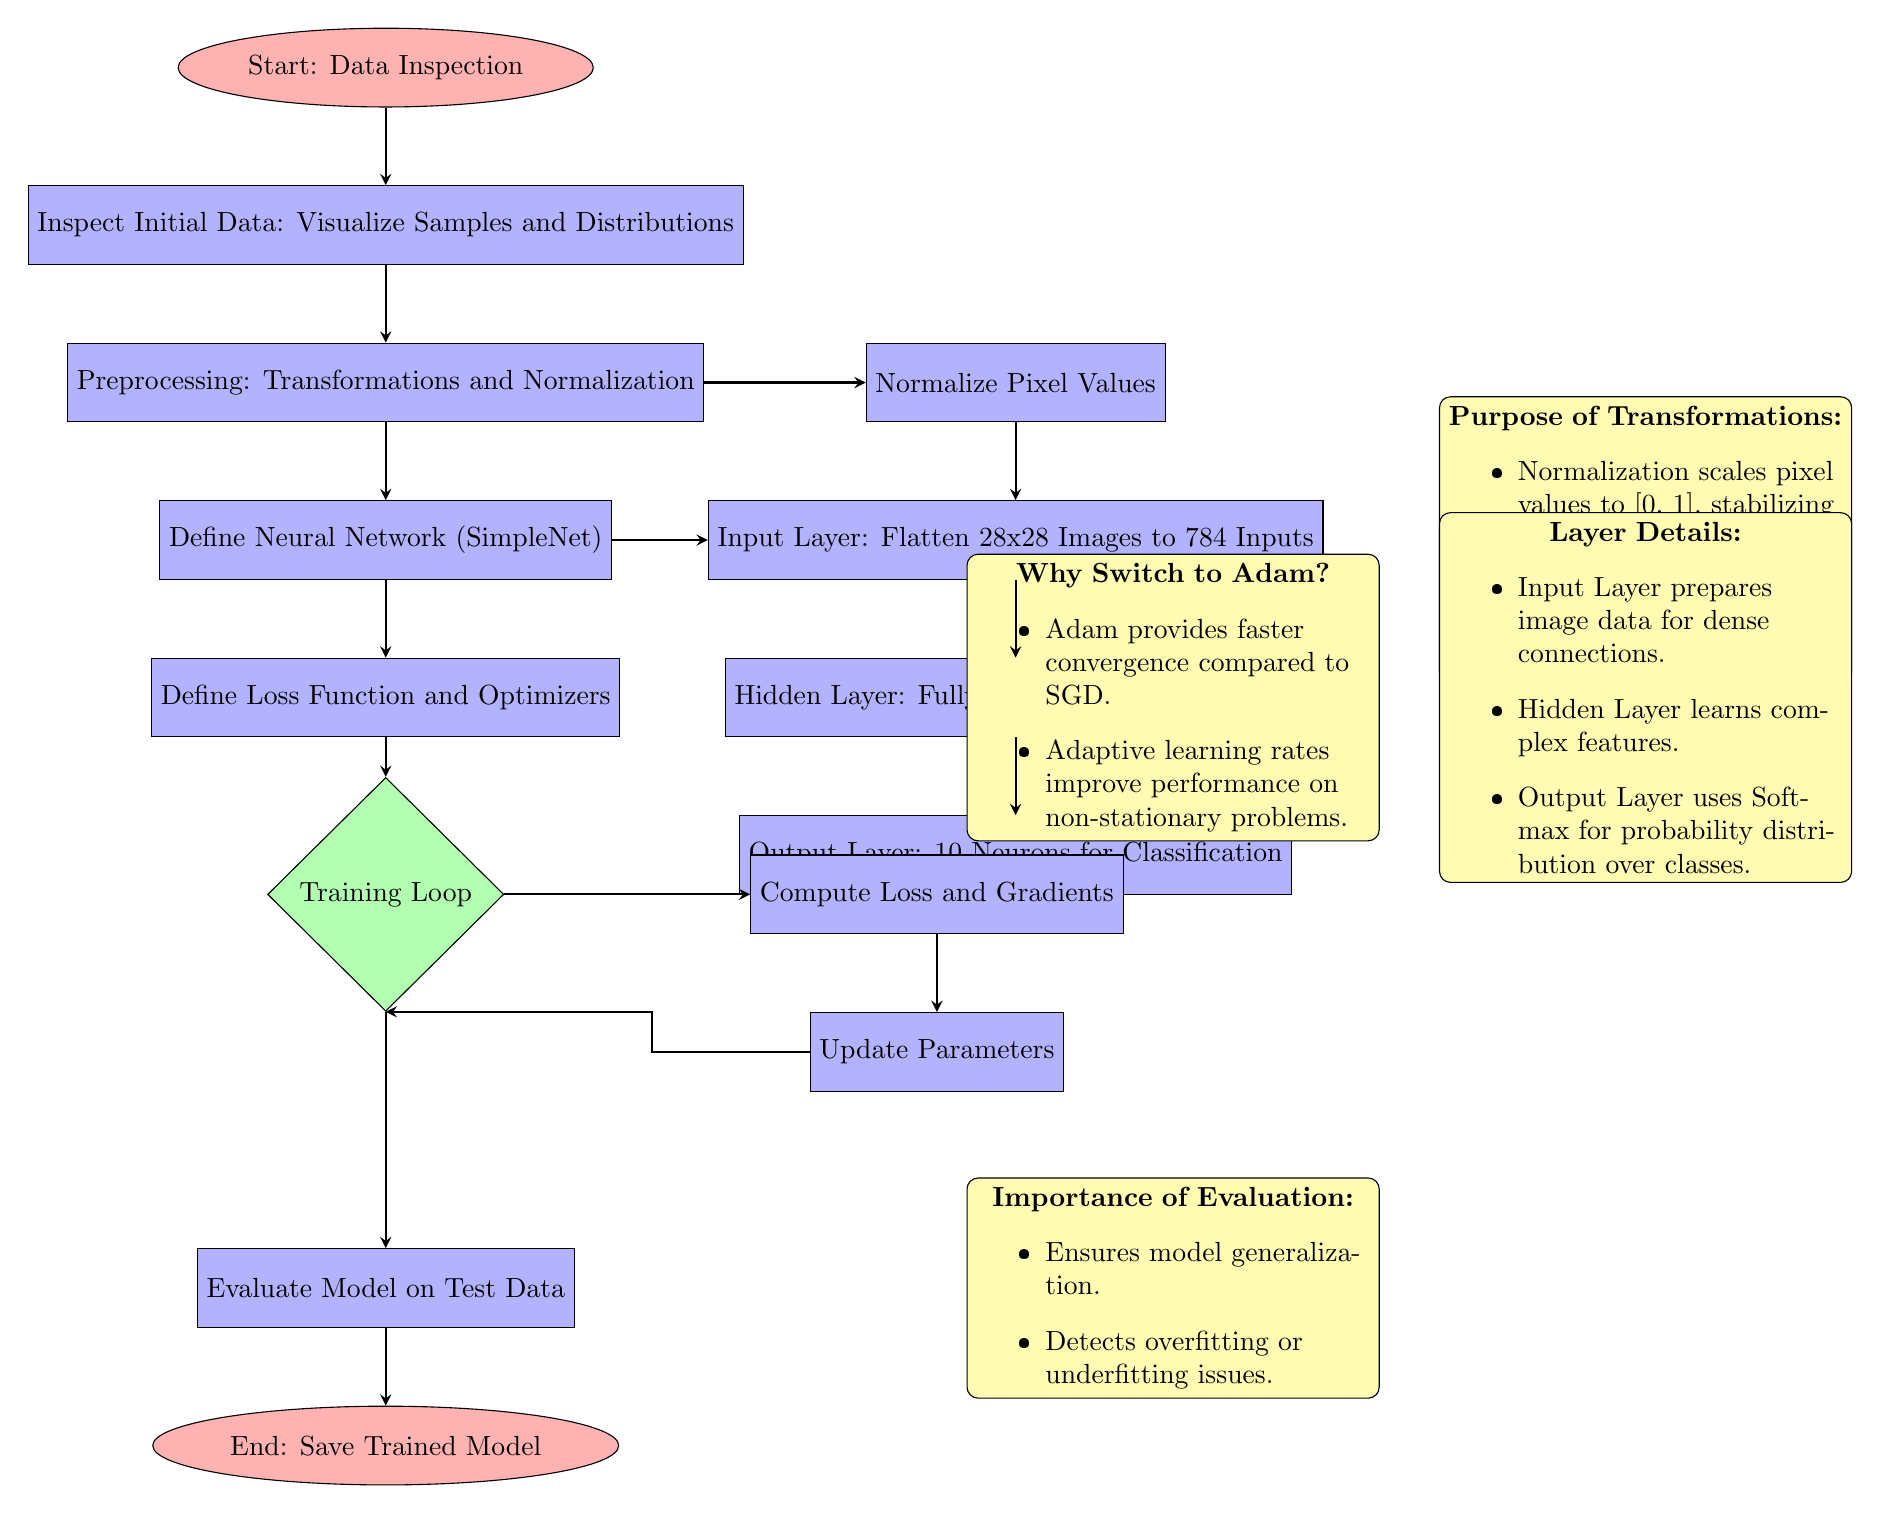
\begin{tikzpicture}[node distance=2cm]

% Start Node
\node (start) [startstop] {Start: Data Inspection};

% Data Inspection Node
\node (inspect) [process, below of=start] {Inspect Initial Data: Visualize Samples and Distributions};

% Preprocessing Breakdown
\node (preprocess) [process, below of=inspect] {Preprocessing: Transformations and Normalization};
\node (normalize) [process, right of=preprocess, xshift=6cm] {Normalize Pixel Values};
\node (augment) [process, below of=normalize] {Data Augmentation: Random Rotations, Flips};
\node (notePreproc) [note, right of=augment, xshift=6cm] {
\textbf{Purpose of Transformations:}
\begin{itemize}
    \item Normalization scales pixel values to [0, 1], stabilizing gradient calculations.
    \item Augmentation increases dataset diversity, reducing overfitting.
\end{itemize}
};

% Define Network Node
\node (defineNet) [process, below of=preprocess] {Define Neural Network (SimpleNet)};

% Layers Breakdown
\node (inputLayer) [process, right of=defineNet, xshift=6cm] {Input Layer: Flatten 28x28 Images to 784 Inputs};
\node (hiddenLayer) [process, below of=inputLayer] {Hidden Layer: Fully Connected (128 Neurons)};
\node (outputLayer) [process, below of=hiddenLayer] {Output Layer: 10 Neurons for Classification};
\node (noteLayers) [note, right of=hiddenLayer, xshift=6cm] {
\textbf{Layer Details:}
\begin{itemize}
    \item Input Layer prepares image data for dense connections.
    \item Hidden Layer learns complex features.
    \item Output Layer uses Softmax for probability distribution over classes.
\end{itemize}
};

% Loss and Optimizer Node
\node (defineLoss) [process, below of=defineNet] {Define Loss Function and Optimizers};

% Training Loop Decision
\node (trainLoop) [decision, below of=defineLoss, yshift=-0.5cm] {Training Loop};

% Compute Loss Node
\node (computeLoss) [process, right of=trainLoop, xshift=5cm] {Compute Loss and Gradients};

% Update Parameters Node
\node (updateParams) [process, below of=computeLoss] {Update Parameters};

% Evaluation Node
\node (evaluate) [process, below of=trainLoop, yshift=-3cm] {Evaluate Model on Test Data};

% Save Model Node
\node (saveModel) [startstop, below of=evaluate] {End: Save Trained Model};

% Notes
\node (noteSGD) [note, right of=defineLoss, xshift=8cm] {
\textbf{Why Switch to Adam?}
\begin{itemize}
    \item Adam provides faster convergence compared to SGD.
    \item Adaptive learning rates improve performance on non-stationary problems.
\end{itemize}
};

\node (noteEval) [note, right of=evaluate, xshift=8cm] {
\textbf{Importance of Evaluation:}
\begin{itemize}
    \item Ensures model generalization.
    \item Detects overfitting or underfitting issues.
\end{itemize}
};

% Arrows
\draw [arrow] (start) -- (inspect);
\draw [arrow] (inspect) -- (preprocess);
\draw [arrow] (preprocess) -- (defineNet);
\draw [arrow] (defineNet) -- (defineLoss);
\draw [arrow] (defineLoss) -- (trainLoop);
\draw [arrow] (trainLoop.east) -- (computeLoss.west);
\draw [arrow] (computeLoss) -- (updateParams);
\draw [arrow] (updateParams.west) -- ++(-2,0) |- (trainLoop.south);
\draw [arrow] (trainLoop.south) -- (evaluate.north);
\draw [arrow] (evaluate) -- (saveModel);

% Preprocessing Breakdown Connections
\draw [arrow] (preprocess.east) -- (normalize.west);
\draw [arrow] (normalize) -- (augment);

% Layers Breakdown Connections
\draw [arrow] (defineNet.east) -- (inputLayer.west);
\draw [arrow] (inputLayer) -- (hiddenLayer);
\draw [arrow] (hiddenLayer) -- (outputLayer);

\end{tikzpicture}

\section*{Explanation of Modifications}

\subsection*{Data Inspection and Preprocessing}
Before starting the training process, it is crucial to inspect the initial dataset. Visualizing sample images and distributions helps in understanding:
\begin{itemize}
    \item Data quality: Identifying corrupted or mislabeled samples.
    \item Distribution: Ensuring balanced class representation.
\end{itemize}

Transformations applied during preprocessing include:
\begin{itemize}
    \item \textbf{Normalization:} Rescales pixel values from [0, 255] to [0, 1]. This stabilizes gradient calculations during backpropagation.
    \item \textbf{Data Augmentation:} Random rotations and flips artificially expand the dataset, improving generalization by reducing overfitting.
\end{itemize}

\subsection*{Neural Network Layers}
The architecture of the neural network is designed to balance simplicity and performance for the MNIST dataset:
\begin{itemize}
    \item \textbf{Input Layer:} Flattens 28x28 pixel images into a single vector of 784 features, preparing data for dense connections.
    \item \textbf{Hidden Layer:} A fully connected layer with 128 neurons and activation functions to capture complex features from the input data.
    \item \textbf{Output Layer:} Contains 10 neurons (one for each digit class) and applies the Softmax activation function to output a probability distribution.
\end{itemize}

\subsection*{Switch from SGD to Adam Optimizer}
SGD is a reliable optimizer but can struggle with convergence on complex datasets or non-stationary problems. By switching to Adam:
\begin{itemize}
    \item The training process adapts learning rates per parameter, which accelerates convergence.
    \item It combines the benefits of momentum and RMSprop, improving stability and efficiency.
\end{itemize}

\subsection*{Evaluation and Generalization}
Regular evaluation during training ensures that the model generalizes well to unseen data. This step is crucial to avoid overfitting, especially in smaller datasets like MNIST.

\end{document}